\documentclass[conference]{IEEEtran}
\IEEEoverridecommandlockouts
% The preceding line is only needed to identify funding in the first footnote. If that is unneeded, please comment it out.

\usepackage{booktabs}
\usepackage{amsmath,amssymb,amsfonts, mathabx}
% \usepackage[backend=biber,style=alphabetic,sorting=ynt]{biblatex}
% \addbibresource{sample.bib} %Import the bibliography file
\usepackage{enumitem}
\usepackage{algorithmic}
\usepackage{physics}
\usepackage{graphicx}
\usepackage{textcomp}
\usepackage[colorlinks=true, allcolors=black]{hyperref}
\usepackage{xcolor}
\usepackage{multirow}
\usepackage[c1]{optidef}
\def\BibTeX{{\rm B\kern-.05em{\sc i\kern-.025em b}\kern-.08em
    T\kern-.1667em\lower.7ex\hbox{E}\kern-.125emX}}
\begin{document}
\title{Model Predictive Control for Waypoint Tracking Mini-quadcopters\\}
\author{\IEEEauthorblockN{Akash John Subash}
\IEEEauthorblockA{\textit{M.Sc. Embedded Systems Engineering}}
}
\maketitle

\begin{abstract}
This report describes a real-time waypoint tracking Model Predictive Control (MPC) formulation for the crazyFlie 2.1 mini quadcopters. It subsequently proposes a trajectory tracking scheme achieved by a path parametric model reformulation using the Frenet-Serret transforms while retaining convex geometric collision constraints in the Cartesian coordinate frame.

\end{abstract}

\section{Introduction}\label{Introduction}
The optimal controls computed offboard using MPC are fed to the crazyFlie, with the intention to overtake a second quadcopter (henceforth referred to as obstacle). The crazyFlie is an agile, underactuated platform for which we specify sufficiently accurate dynamics.

Section \hyperref[Section2]{II} describes the dynamics of the crazyFlie 2.1 quadcopter using Ordinary Differential Equations (ODE). Section \hyperref[Section3]{III} details the optimal control problem, its Non-Linear Program (NLP) and Section \hyperref[Section4]{IV} the control scheme. Section \hyperref[Section5]{V} presents the results of simulation and flight tests and Section \hyperref[Section6]{VI} subsequently outlines the ongoing reformulation for trajectory tracking and its foreseen timeline.
\section{System Modelling}\label{Section2}
\begin{figure}[htbp]
	\centerline{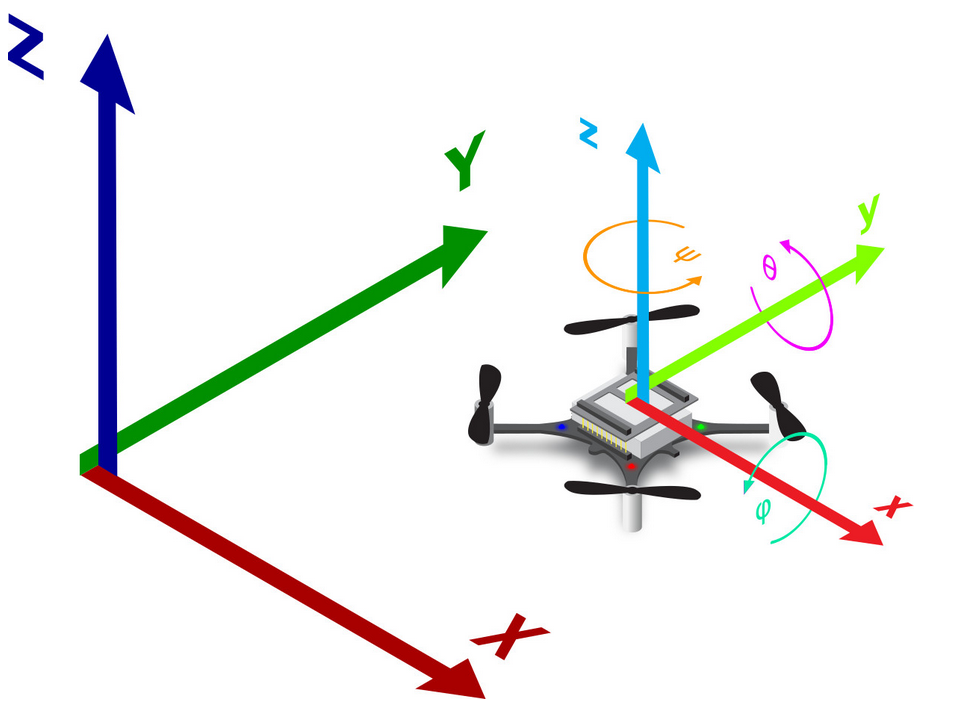
\includegraphics[scale = 0.4]{figures/ordinate.png} }
	\caption{Reference coordinate system [1]}
	\label{Fig1}
\end{figure}
As depicted in \hyperref[Fig1]{Fig. 1}, a body frame located at the center of mass of the quadcopter aligned with the East-North-Up inertial frame is used here, with $\varphi$, $\theta$, $\psi$ representing roll, pitch and yaw Euler angles respectively.

\subsection{Dynamic Model}\
The state ${\zeta\,\in\,\mathbb{R}\,\mathrm{^{13}}}$ of the drone described by position ${p = (x, y, z)^{\mathrm{T}}}$ and transalational velocities ${v = (v_x, v_y, v_z)^\mathrm{T}}$ in the inertial frame $\mathcal{I}$, attitude in quaternion ${q = (q_{0}, q_{1}, q_{2}, q_{3})^{\mathrm{T}}}$, and angular velocities ${\omega = (\omega_{\phi}, \omega_{\theta}, \omega_{\psi})^{\mathrm{T}}}$ in the body frame $\mathcal{B}$. Its non-linear dynamics adapted from \cite{carlos_efficient_2020} are given by the ODEs

\begin{align}
\dot{\zeta} &= \begin{bmatrix}
	\dot{p} \\
	\dot{q}\\
	\dot{v}\\
	\dot{\omega}
\end{bmatrix} =
\begin{bmatrix}
    v \\
    \dfrac{1}{2}q\times \omega\\
    \dfrac{1}{m}F - S\mathrm{^{T}}g1_z - \dfrac{C_d}{m} v\\
    J\mathrm{^{-1}}\left(M - \omega \times J \omega\right)
\end{bmatrix}.
\end{align}

The model parameters described in \hyperref[table1]{Table I} are used in conjunction with the quaternion rotation matrix ${S\,\in\,\mathbb{R}\,\mathrm{^{3\times3}}}$, external force matrix ${F\,\in\,\mathbb{R}\,\mathrm{^{3\times1}}}$, external momentum matrix ${M\,\in\,\mathbb{R}\,\mathrm{^{3\times1}}}$, and moment of inertia matrix ${J\,\in\,\mathbb{R}\,\mathrm{^{3\times3}}}$ as

\begin{align}
	S &= 2 \cdot
	\begin{bmatrix}
		q_{0}^{2} + q_{1}^{2} - \dfrac{1}{2} &
		q_1 q_2 - q_0 q_3 &
		q_0 q_2 + q_2 q_3 \\
		q_0 q_3 + q_1 q_2 &
		q_{0}^{2} + q_{2}^{2} - \dfrac{1}{2} &
		q_2 q_3 - q_0 q_1 \\
		q_1 q_3 - q_0 q_2 &
		q_0 q_1 + q_2 q_3 &
		q_{0}^{2} + q_{3}^{2} - \dfrac{1}{2}\\
	\end{bmatrix}
\end{align}

\begin{align}
	F &=
	\begin{bmatrix}
		0 \\
		0 \\
		C_t(\Omega_1\mathrm{^{2}} + \Omega_2\mathrm{^{2}} + \Omega_3\mathrm{^{2}} + \Omega_4\mathrm{^{2}})\\
	\end{bmatrix}
\end{align}

\begin{align}
	J &=
	\begin{bmatrix}
		I_{x} & 0 & 0\\
		0 & I_{y} & 0\\
		0 & 0 & I_{z}\\
	\end{bmatrix}
\end{align}

\begin{align}
	M &=
	\begin{bmatrix}
		\frac{1}{\sqrt{2}}\,dC_t(-\Omega_1\mathrm{^{2}} - \Omega_2\mathrm{^{2}} + \Omega_3\mathrm{^{2}} + \Omega_4\mathrm{^{2}})\\
		\frac{1}{\sqrt{2}}\,dC_t(-\Omega_1\mathrm{^{2}} + \Omega_2\mathrm{^{2}} + \Omega_3\mathrm{^{2}} - \Omega_4\mathrm{^{2}})\\
		C_d(-\Omega_1\mathrm{^{2}} + \Omega_2\mathrm{^{2}} - \Omega_3\mathrm{^{2}} + \Omega_4\mathrm{^{2}})
	\end{bmatrix}.
\end{align}
Given the possibility to individually change the angular velocities of the propellers, the control vector is defined as: \\
$u$ := ($\Omega_{1}$, $\Omega_{2}$, $\Omega_{3}$, $\Omega_{4}$)$\mathrm{^{T}}$ $\in$ $\mathbb{R}\mathrm{^{4}}$

\begin{table}[htbp]
	\small
	\begin{center}
		\begin{tabular}{lccccl}\toprule
			\textbf{Description} &  \textbf{Symbol}\\
			\midrule
            $\mathrm{Mass\,of\,the\,drone} \,m$ & $\mathrm{31 \cdot 10^{-3}\,\mathrm{kg}}$  \\
			$\mathrm{Drone\,arm\,length} \,d$ & $46 \cdot \mathrm{10^{-3}}\,\mathrm{m}$ \\
			$\mathrm{Inertial\,moment} \,I_{x}$ & $1.395 \cdot\,\mathrm{10^{-5}} \mathrm{kg\,m^2}$ \\
            $\mathrm{Inertial\,moment} \,I_{y}$ & $1.395 \cdot\,\mathrm{10^{-5}} \mathrm{kg\,m^2}$ \\
            $\mathrm{Inertial\,moment} \,I_{z}$ & $2.173 \cdot\,\mathrm{10^{-5}} \mathrm{kg\,m^2}$ \\
            $\mathrm{Coefficient\,of\,drag} \,C_d$ & $\mathrm{7.93 \cdot 10^{-12}}\,\mathrm{N\,RPM^{-2}}$ \\
			$\mathrm{Coefficient\,of\,thrust} \,C_t$ & $\mathrm{3.25 \cdot 10^{-10}}\,\mathrm{N\,RPM^{-2}}$ \\
			$\mathrm{Gravitational\,acceleration} \,g$ & $\mathrm{9.81 \cdot\,m\,s^{-2}}$ \\
			\bottomrule
		\end{tabular}
	\end{center}
	\caption{Parameters of the model}
	\label{table1}
\end{table}

\begin{figure*}[htbp]
	\centerline{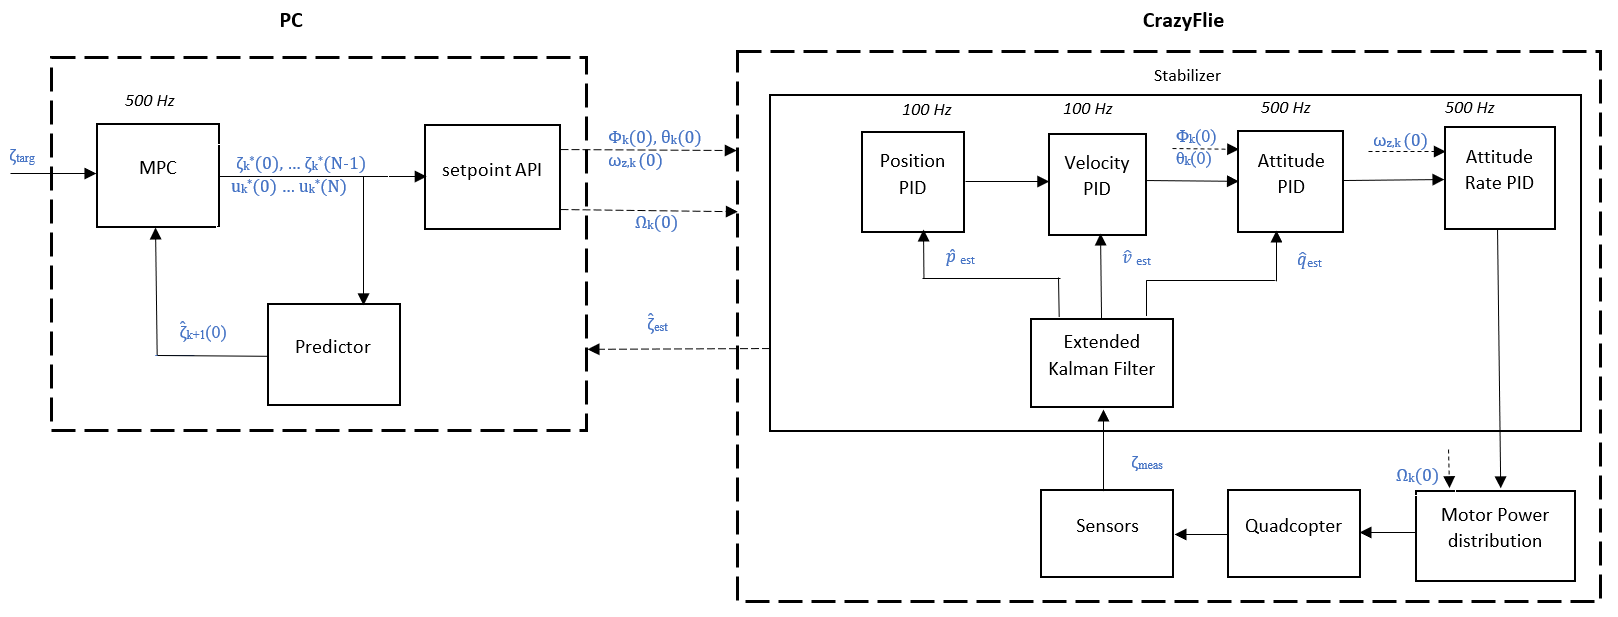
\includegraphics[scale = 0.6]{figures/Screenshot_OL.png} }
	\caption{Open loop control architecture }
	\label{Fig2}
\end{figure*}

\section{Problem Formulation}\label{Section3}

In this section, the discretized Optimal Control Problem (OCP) and its constrained Non-Linear Program (NLP) are defined using direct multiple shooting \cite{bock_multiple_1984} to discretize the underlying continuous-time OCP.

\subsection{Optimal Control Problem}

\par The setpoint tracking NLP defined for an initial state $\bar{\zeta_0}$ with the quadcoptor positioned at $p_0 = (0, 0, 0.5)^T$, and obstacle at $p_\mathrm{b} = (x_\mathrm{b}, y_\mathrm{b}, z_\mathrm{b})^{\mathrm{T}}$ is defined as

\begin{mini!}|l|
	{u_0,\zeta_0,..,u_{N-1},\zeta_N}{\sum_{k = 0}^{N-1} L\left(\zeta_{k}, u_k\right)}{{\label{OCP}}}{}
	\addConstraint{}{\quad \quad \zeta_0 - \bar{\zeta_0}}{=0}
	\addConstraint{}{\quad \quad \zeta_{k+1} - F(\zeta_k, u_k)}{=0,\hspace{0.9em} k=0,\ldots,N-1}
	\addConstraint{-\overline{v} }{\le \quad v_k }{\le \overline{v},\hspace{0.8em} k=0,\ldots,N-1}
	\addConstraint{-\overline{\omega} }{\le \quad \omega_k }{\le \overline{\omega},\hspace{0.8em} k=0,\ldots,N-1}
	\addConstraint{3\,\mathrm{d} }{\le \quad \lVert p_k - p_{\mathrm{b}} \rVert}{\qquad, \hspace{0.8em} k=0,\ldots,N-1}
	\addConstraint{\underline{u} }{\le \quad u_k}{\le \overline{u},\hspace{0.8em} k=0,\ldots,N-1}.
\end{mini!}

\begin{flushleft}
$\bar{\zeta_0}$ \hspace{0.18in}= $(0, 0, 0.5, 1, 0, 0, 0, 0, 0, 0, 0, 0, 0)^T$\\
$\zeta_{\mathrm{trg}}$ \hspace{0.08in}= $( 1, 1, 1, 1, 0, 0, 0, 0, 0, 0, 0, 0, 0)^T$\\
$\overline{v}$ \hspace{0.22in}= $(0.25,0.25,0.25)^T$\\
$\overline{\omega}$ \hspace{0.22in}= $(\frac{\pi}{4},\frac{\pi}{4},\frac{\pi}{4})^T$\\
$\overline{u}$ \hspace{0.22in}= $(2.2, 2.2, 2.2, 2.2)^T \cdot 10^{3}$\\
$p_\mathrm{b}$ \hspace{0.18in}= $(0.5, 0.5, 0.5)^T$\\
\end{flushleft}

\par Here, $(\zeta^{d}_{0}, \dots, \zeta^{d}_{N})$, and $(u_0, \dots, u_{N-1})$ denote the discrete-time state and control trajectories for the horizon length $N$ respectively, and $\phi(\zeta^{d}_k, u_k)$, the discretized dynamics with an RK4 integrator.

 $Q = \mathrm{diag}([Q_{p}, Q_{\alpha}])$ $\in$ $\mathbb{R}^{n_{\zeta} \cdot n_{\zeta}}$ and $R$ $\in$ $\mathbb{R}^{n_{u} \cdot n_{u}}$ are positive definite weighting matrices, tuned experimentally for the specific flight path.

 \begin{table}[b!]
    \small
	\begin{center}
        \begin{tabular}{lc}\toprule
		    \textbf{Quantity} & \textbf{Value}\\
            \midrule
            sampling time $\tau_{s}$ & 20 $\cdot$ $10^{-2}\,\mathrm{s}$ \\
            measurement delay $\tau_{m}$ & 7 $\cdot$ $10^{-3}\,\mathrm{s}$ \\
            actuation delay $\tau_{a}$ & 3 $\cdot$ $10^{-3}\,\mathrm{s}$ \\
            state weights $Q_{p}$ & $(120, 100, 100, 10^{-3}, 10^{-3},10^{-3})$\\
			state weights $Q_{\alpha}$ & $(1, 1, 1, 1, 10^{-5}, 10^{-5}, 10^{-5})$\\
            control weights $R$ & $\mathrm{diag}(\, [1, \,1, \,1, \,1]\,)$\\
		    horizon length $N$ & 20\\
            \bottomrule
		\end{tabular}
	\end{center}
    \caption{Parameters for NMPC formulation. Units in SI units, if not specified explicitly.}
    \label{table2}
\end{table}

\section{Experimental Results }\label{Section4}
Using IPOPT \cite{wachter_implementation_2006} as the interior point NLP solver, the estimated state from the Extended Kalman filter onboard the Crazyflie sampled at 50 Hz, was fed back with delay compensation for closed-loop control. The sampling rate was determined by the lower bound on the achievable computation time of the solver. Using MPC to control the system, an instance of (2) is solved iteratively at each sampling time point, with the current value of the state estimate $\zeta_k$.

The closed loop architecture differs from Figure 2, only in the feedback path, where the predictor computes $\hat{\zeta}_{k+1}$ from $\hat{\zeta}_{\mathrm{est}}$ instead of $\zeta^*_{k}$.

\subsection{Delay Compensation}

The round trip delay is computed as the sum of radio communication latency between the off-board processor and the quadcopter, and NLP solution times ( $\tau_{tr}$ = $\tau_{t}$ + $\tau_{r}$ + $\tau_{c}$). The inherent challenge of measuring one-way latency is accounted for and handled to retain optimality as in \cite{carlos_efficient_2020} by introducing a delay compensation block marked as the predictor in Figure 2.

\subsection{Closed-loop Control}\label{Section5}

A challenge to consider while moving from numerical plant simulations to hardware flights was the round trip delay $\tau_{tr}$. The choice of
$\tau_s$ was foreseen to provide a good tradeoff between the solution optimality and solution time $\tau_{c}$.
$\tau_{tr}$ was found to be dominated by $\tau_{c}$, which is dependant on the choice of the solver, and the discretization interval ($\tau_s$), and more importantly, the OCP formulation.

\begin{figure}[t!]
    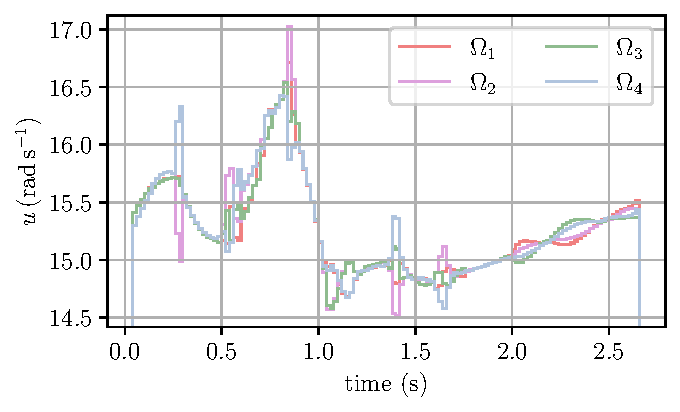
\includegraphics[width=0.48\textwidth]{figures/u.pdf}
    \caption{Control $(u)$ for active collision constraints, with a numerical plant simulation}  \label{fig_comp_zeta_u_AGV}
\end{figure}

Since the choice of $N$ trades off control trajectory smoothness and $\tau_{c}$, the naively formulated collision constraint compromises real-time feasibility when active.

The average closed-loop iteration times were $\tau_{c}$ = 40 ms, and $\tau_{c}$ = 100 ms without and with active collision constraints on an Intel i7-8750H processor @2.2Ghz running Windows.
\section{Proposal}\label{Section6}
\par The superior convergence properties of the spatial reformulation for trajectory tracking problems introduced in \cite{werling_invariant_2010}, is partially utilized for drone dynamics in \cite{arrizabalaga_towards_2022}. Although position derivates are sufficient for the trajectory tracking problem here, collision constraints would additionally need to parametrize the heading angles. To retain convex constraint guarantees using the lifted and direct elimination controllers as in \cite{reiter_frenet-cartesian_2023}, we need to specify the full transforms in 3 dimensions using the Frenet-Serret theorem. Subsequently, the constraint tightening \cite{reiter_progressive_nodate} shows promise for improved geometric specification for the demanding geometric collision constraints, while avoiding slacks.
Verifying observer design and delay modeling in the feedback path could be simplified with a data-driven high-fidelity model \cite{llanes_crazysim_nodate} in simulation. To achieve a real-time feasible scheme we aim to use hardware-tailored linear algebra libraries \cite{frison_blasfeo_2018} in acados \cite{verschueren_acados_2020} with the real-time iteration \cite{gros_linear_2020} (RTI) and partial condensing to exploit the structured QP subproblem \cite{frison_hpipm_2020}.
\begin{figure}[t!]
	\centerline{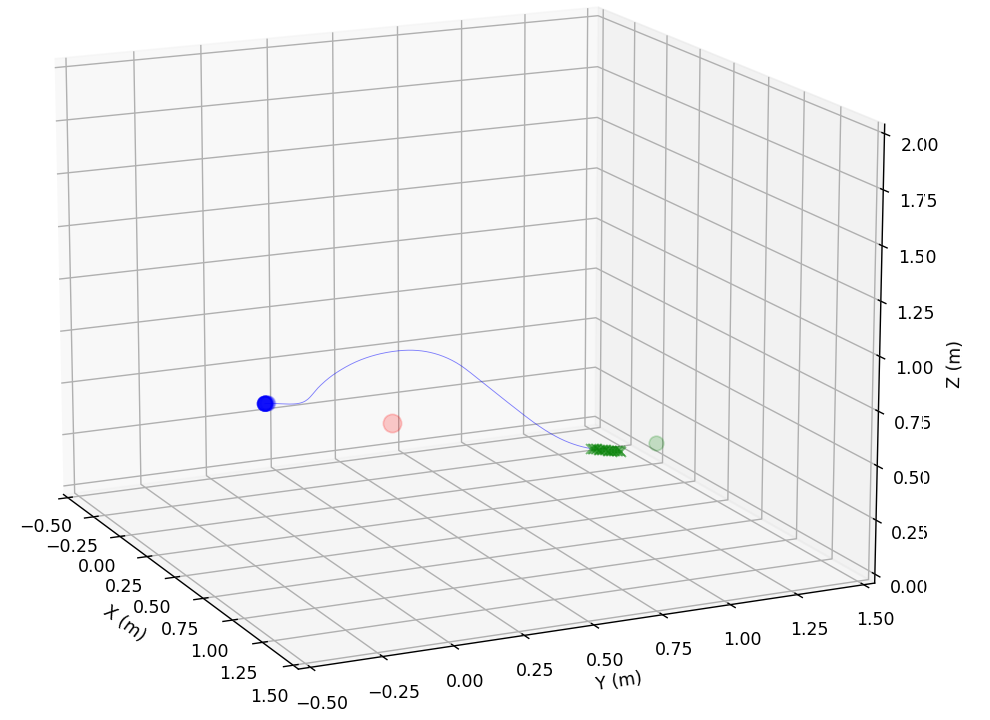
\includegraphics[scale = 0.4]{figures/Screenshot_OLwO_ST.png} }
	\caption{Position vector $(p)$ for active collision constraints, with a numerical plant simulation}
	\label{Fig4}
\end{figure}
\bibliographystyle{ieeetr}
\bibliography{./bibliography/sample.bib}
\end{document}

% git commit --amend
% git rebase -i revision